\documentclass{article}
\iffalse
This file is protected by Copyright. Please refer to the COPYRIGHT file
distributed with this source distribution.

This file is part of OpenCPI <http://www.opencpi.org>

OpenCPI is free software: you can redistribute it and/or modify it under the
terms of the GNU Lesser General Public License as published by the Free Software
Foundation, either version 3 of the License, or (at your option) any later
version.

OpenCPI is distributed in the hope that it will be useful, but WITHOUT ANY
WARRANTY; without even the implied warranty of MERCHANTABILITY or FITNESS FOR A
PARTICULAR PURPOSE. See the GNU Lesser General Public License for more details.

You should have received a copy of the GNU Lesser General Public License along
with this program. If not, see <http://www.gnu.org/licenses/>.
\fi

% TODO: Version numbers?
\usepackage{fancyhdr}
\usepackage{colortbl}
\usepackage{hyperref}
\setcounter{secnumdepth}{0} % No numbers, but import into TOC anyway
% \usepackage{listings}
% \begin{lstlisting}
\usepackage[margin=.75in]{geometry}
\usepackage{microtype}
\usepackage{multirow}
\usepackage{array}
\usepackage{indentfirst} % Indent all paragraphs
\usepackage{float}
\usepackage{graphicx}
% \usepackage[table,xcdraw]{xcolor}
\pagestyle{fancy}
\headheight=23pt
\lhead{ANGRYVIPER RX App}
\rhead{ANGRYVIPER Team}
\renewcommand{\headrulewidth}{0pt}
\definecolor{blue}{rgb}{.7,.8,.9}
\usepackage{ifpdf}
\ifpdf
\setlength{\pdfpagewidth}{8.5in}
\setlength{\pdfpageheight}{11in}
\else
\fi
\usepackage{pifont}
% This block is to make sure there is 3cm min at the bottom of a page before a new section or subsection is allowed to start. Otherwise, next page.
% Modified from http://tex.stackexchange.com/a/152278
\usepackage{etoolbox}
\newskip\mfilskip
\mfilskip=0pt plus 3cm\relax
\newcommand{\mfilbreak}{\vspace{\mfilskip}\penalty -200%
  \ifdim\lastskip<\mfilskip\vspace{-\lastskip}\else\vspace{-\mfilskip}\fi}
\pretocmd{\section}{\mfilbreak}{}{}
\pretocmd{\subsection}{\mfilbreak}{}{}
% end [sub]section pushes

\usepackage{tabularx}
\usepackage{pdflscape} % for landscape view
% These define tabularx columns "C" and "R" to match "X" but center/right aligned
\newcolumntype{C}{>{\centering\arraybackslash}X}
\newcolumntype{R}{>{\raggedleft\arraybackslash}X}
\newcolumntype{P}[1]{>{\centering\arraybackslash}p{#1}}

\usepackage{rotating}
\newcommand{\todo}[1]{\textcolor{red}{TODO: #1}\PackageWarning{TODO:}{#1}}
% \parindent=20pt
% \hangindent=0.7cm
\graphicspath{ {figures/} }
\definecolor{drkgreen}{rgb}{0,.6,0}
\begin{document}

\tableofcontents
\vspace{1pc}
\hrule
\section{Document Scope}
\noindent This document describes the ANGRYVIPER RX App demo application. It includes a description of the RX App application and instructions on how to setup the hardware and build, execute, and test the software.

\section{Supported Hardware Setups}
\noindent This app may be used on the Matchstiq-Z1, Zedboard/Zipper/MyriadRF combination, x86/Stratix IV GX development kit (230 Edition)/Zipper/MyriadRF combination, and the x86/ML605/Zipper/MyriadRF combination. Note that only one Zipper/MyriadRF may be plugged into the platforms which contain multiple slots. Note also that on x86 host machines with multiple Stratix IV and/or ML605s plugged into PCIe slots, this app will assume that the first found Stratix IV/ML605 has a Zipper/MyriadRF plugged in. The first found Stratix IV/ML605 will be used during execution.

\section{Description}
\noindent A block diagram of the RX app (for Stratix IV GX230 / Zipper on HSMC B specifically) can be seen in Figures \ref{fig:rx_app_left} and \ref{fig:rx_app_right}. Complex samples from the ADC are ingested into the FPGA, processed, potentially timestamped, and written to file.
\pagebreak
\begin{landscape}
	\begin{figure}[H]
	 	\centering
		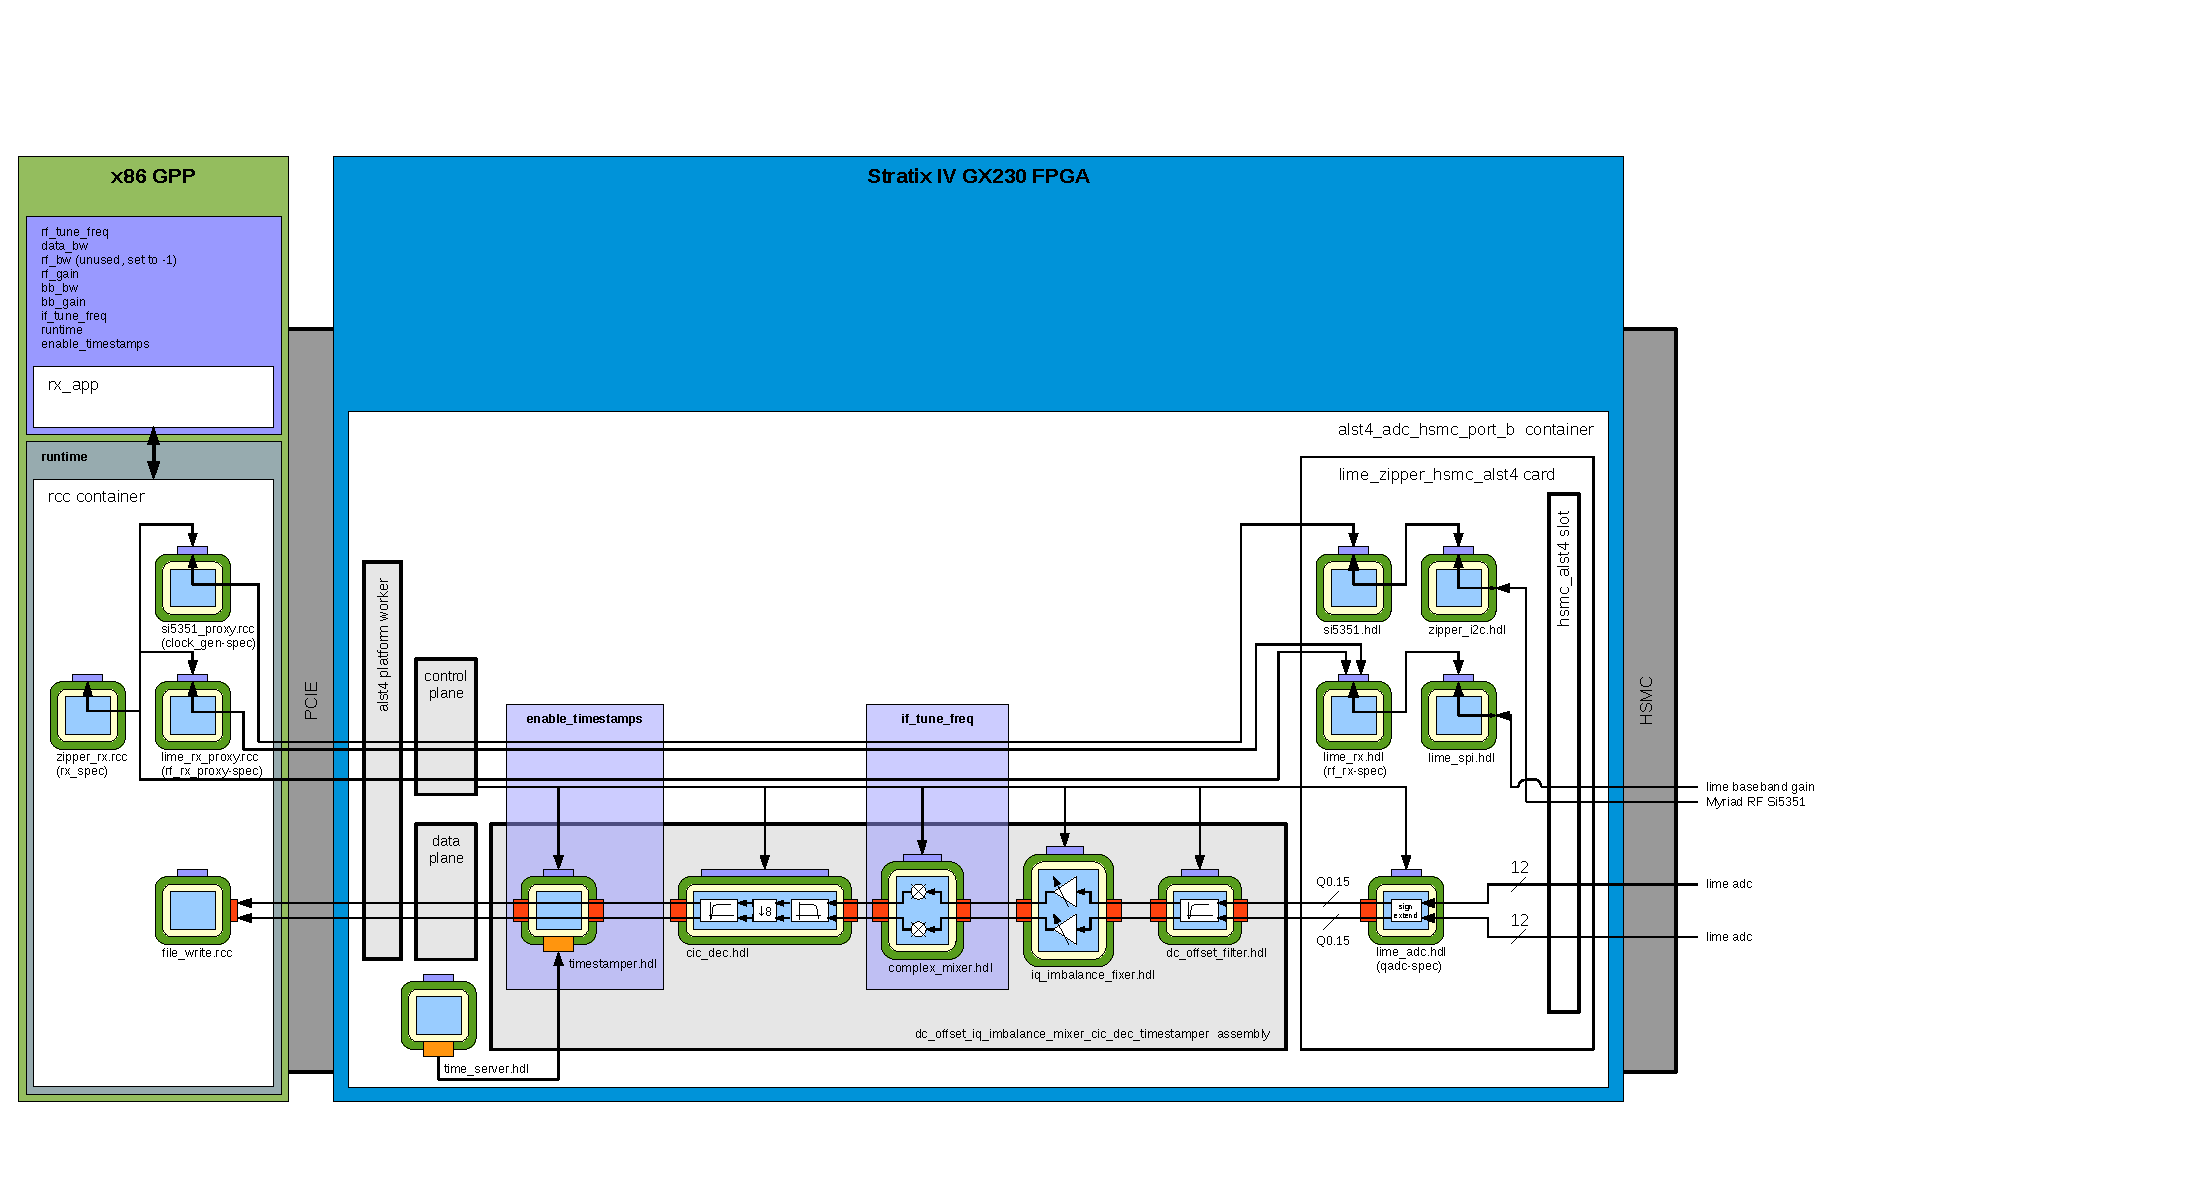
\includegraphics[scale=.750, trim={0 0 6cm 0}]{rx_app_left}
		\caption{RX App Block Diagram for Stratix IV GX230 with Zipper on HSMC B (1/2)}
		\label{fig:rx_app_left}
	\end{figure}
	\begin{figure}[H]
	 	\centering
		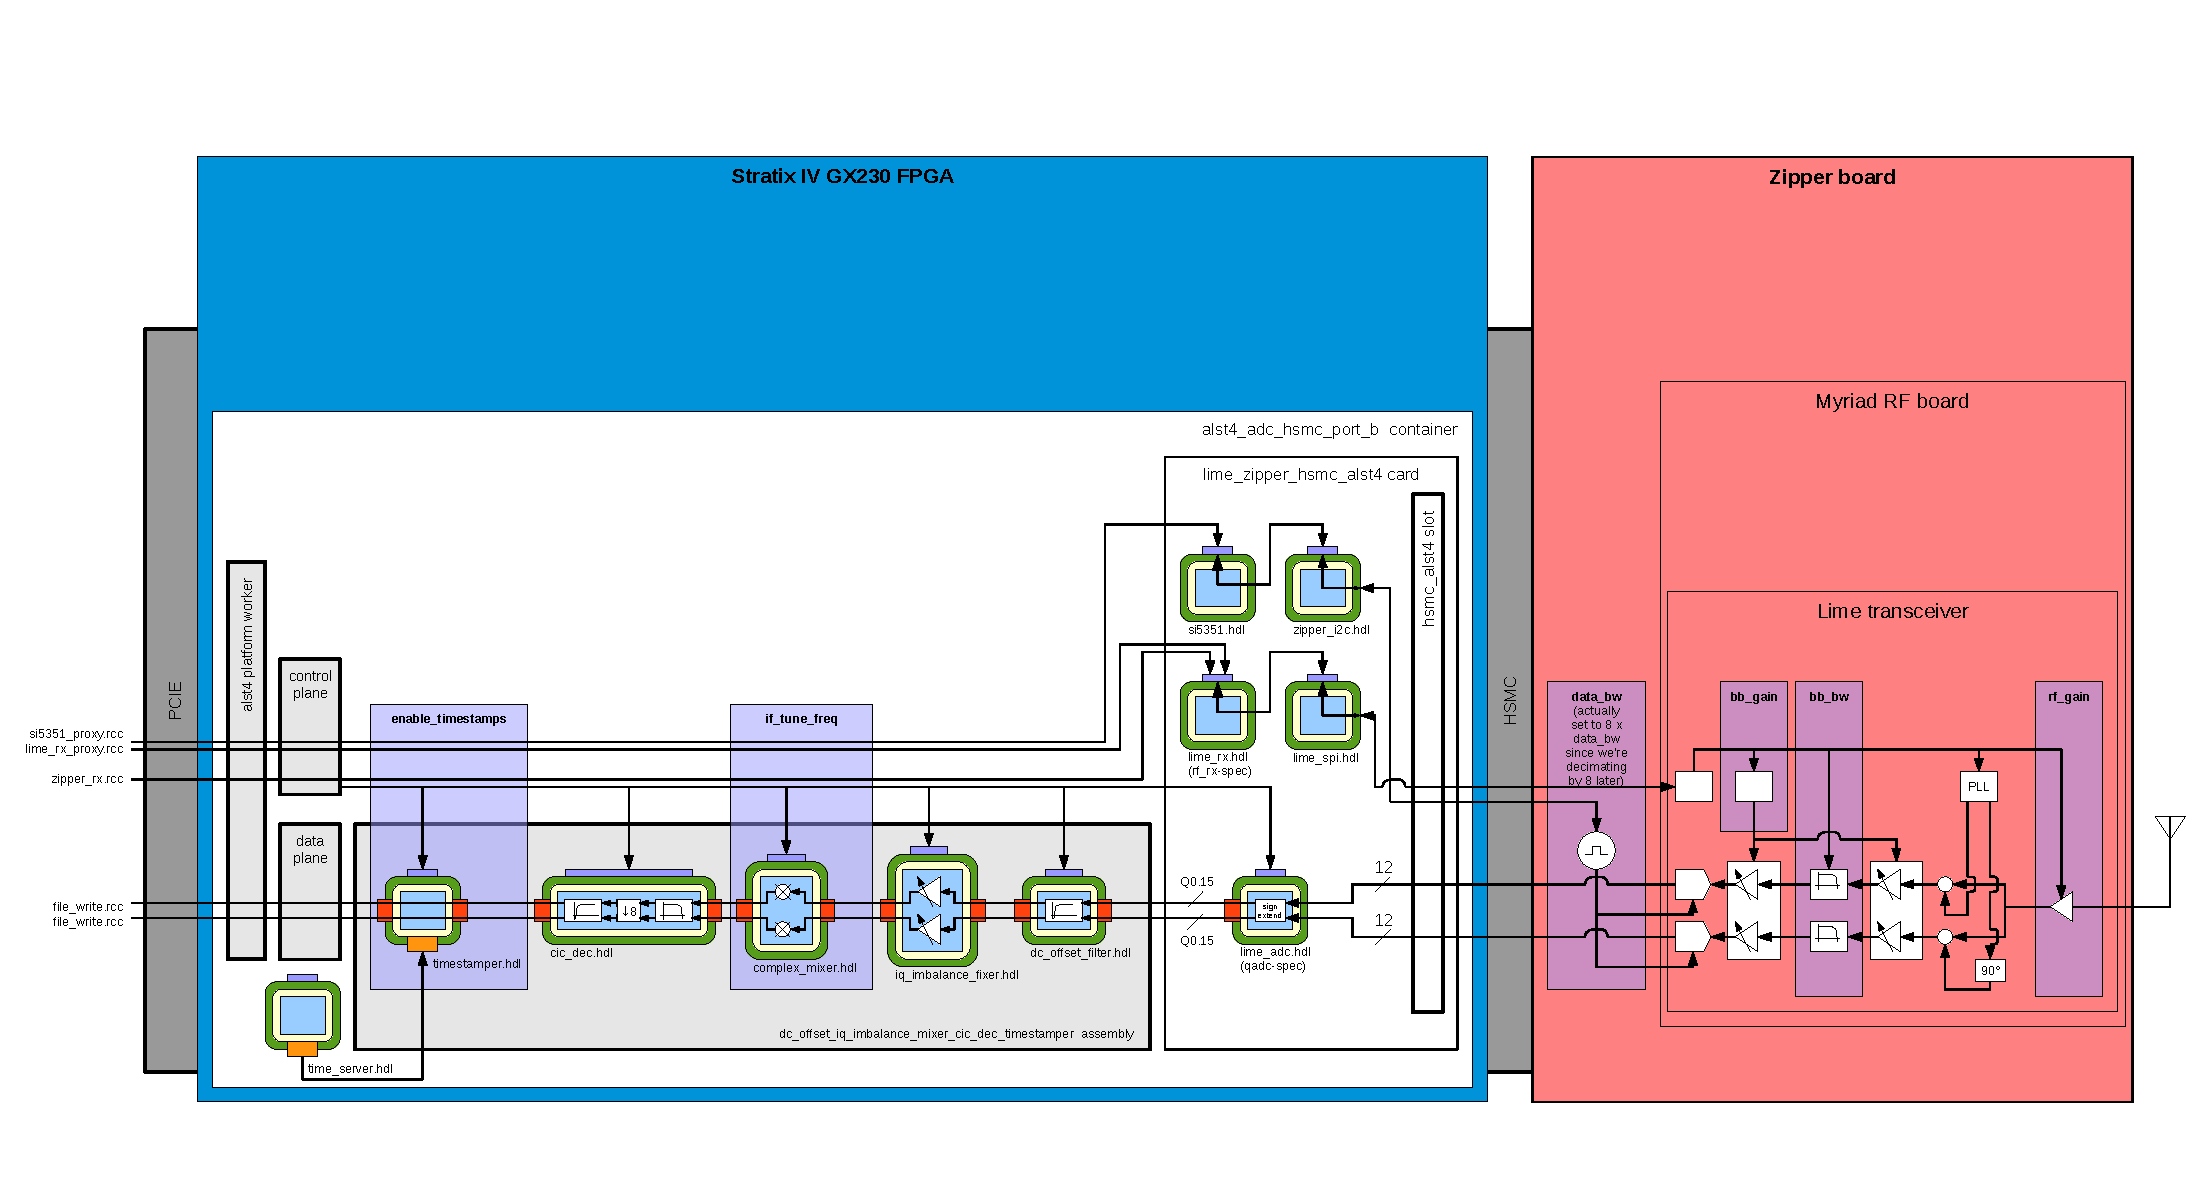
\includegraphics[scale=.65, trim={0 0 1cm 0}]{rx_app_right}
		\caption{RX App Block Diagram for Stratix IV GX230 with Zipper on HSMC B (2/2)}
		\label{fig:rx_app_right}
	\end{figure}
\end{landscape}

\section{Building the Application}
\subsection{Dependencies}
\noindent The following components, sorted by component library name, must be built prior to building RX app. See Appendix A for the parameter configurations used in the application, and see the individual component datasheets for more information and build instructions.\par\bigskip
	\begin{minipage}[t]{.5\textwidth}
	\textbf{Matchstiq-Z1}
	\begin{itemize}
		\item ocpi
			\subitem file\_write.rcc
		\item ocpi.assets.util\_comps
			\subitem timestamper.hdl
		\item ocpi.assets.dsp\_comps
			\subitem cic\_dec.hdl
			\subitem complex\_mixer.hdl
			\subitem iq\_imbalance\_fixer.hdl
			\subitem dc\_offset\_filter.hdl
		\item ocpi.devices
			\subitem lime\_adc.hdl
			\subitem lime\_rx\_proxy.rcc
			\subitem lime\_rx.hdl
			\subitem lime\_spi.hdl
		\item ocpi.assets.devices
			\subitem pca9535.hdl
			\subitem si5338\_proxy.rcc
			\subitem si5338.hdl
			\subitem tmp100\_proxy.rcc
			\subitem tmp100.hdl
		\item ocpi.assets.platforms.matchstiq\_z1.devices
			\subitem matchstiq\_z1\_rx.rcc
			\subitem matchstiq\_z1\_avr\_proxy.rcc
			\subitem matchstiq\_z1\_avr.hdl
			\subitem matchstiq\_z1\_pca9535\_proxy.rcc
			\subitem matchstiq\_z1\_i2c.hdl
	\end{itemize}
	\end{minipage}
	\begin{minipage}[t]{.5\textwidth}
	\textbf{Zedboard/Stratix IV GX230/ML605 with Zipper}
	\begin{itemize}
		\item ocpi
			\subitem file\_write.rcc
		\item ocpi.assets.util\_comps
			\subitem timestamper.hdl
		\item ocpi.assets.dsp\_comps
			\subitem cic\_dec.hdl
			\subitem complex\_mixer.hdl
			\subitem iq\_imbalance\_fixer.hdl
			\subitem dc\_offset\_filter.hdl
		\item ocpi.devices
			\subitem lime\_adc.hdl
			\subitem lime\_rx\_proxy.rcc
			\subitem lime\_rx.hdl
			\subitem lime\_spi.hdl
			\subitem si5351\_proxy.rcc
			\subitem si5351.hdl
		\item ocpi.assets.devices
			\subitem zipper\_rx.rcc
	\end{itemize}
	\end{minipage}
\newpage

\noindent Additionally, platform support for the Matchstiq-Z1/Zedboard/Stratix IV/ML605 must also be built prior to building the RX app. See the respective Platform Data Sheet for more information and build instructions.
\subsection{HDL Assembly and HDL Container}
\noindent The FPGA portion of the application consists of the dc\_offset\_iq\_imbalance\_mixer\_cic\_dec\_timestamper HDL assembly and the appropriate  Matchstiq-Z1/Zedboard/Stratix IV/ML605 HDL container file. The HDL assembly instances the signal processing and timestamping components. The HDL container has three primary functions in this application:
\begin{itemize}
	\item[1)] Connects HDL assembly input to the ADC hardware for gathering IQ data
	\item[2)] Connects HDL assembly output to the processor for writing data to disk
	\item[3)] Instances command and control SPI/I2C HDL Device Workers required to configure the RF front end
\end{itemize}
\subsection{Performance and Resource Utilization}
\begin{scriptsize}
\begin{tabular}{|P{1.8cm}|c|c|c|c|c|P{1.32cm}|}
\hline
\rowcolor{blue}
Platform               & Device              & Registers & LUTs  & Fmax    & Memory/Special Functions & Design Suite       \\
\hline
Matchstiq-Z1               & XC7Z020-1-CLG484    & 9826     & 9896 & 100 MHz & DSP48E1 = 15             & Vivado 2017.1 \\
\hline
Matchstiq-Z1           & XC7Z020-1-CLG484    & 8375      & 11118 & 100 MHz & DSP48E1 = 15             & ISE 14.7           \\
\hline
ML605 FMC HPC          & XC6VLX240T-1-FF1156 & 13871     & 18195 & 125 MHz & DSP48E1 = 15             & ISE 14.7           \\
\hline
ML605 FMC LPC          & XC6VLX240T-1-FF1156 & 13872     & 18376 & 125 MHz & DSP48E1 = 15             & ISE 14.7           \\
\hline
Stratix IV HSMC Port A & EP4SGX230K-C2-F40   & 41048     & 27072 & 125 MHz & DSP 18x18 = 26           & Quartus Prime 15.1 \\
\hline
Stratix IV HSMC Port B & EP4SGX230K-C2-F40   & 41048     & 27072 & 125 MHz & DSP 18x18 = 26           &  Quartus Prime 15.1 \\
\hline
Zedboard               & XC7Z020-1-CLG484    & 8772     & 8872 & 100 MHz & DSP48E1 = 15             & Vivado 2017.1 \\
\hline
Zedboard               & XC7Z020-1-CLG484    & 7431      & 10231 & 100 MHz & DSP48E1 = 15             & ISE 14.7           \\
\hline
\end{tabular}
\end{scriptsize}
\subsection{Executable}
\noindent The software portion of the application consists of a C++ program written using the OpenCPI C++ API, RCC proxy components for command and control functionality, and the file\_write.rcc RCC App Worker for capturing data. For more implementation details on the command and control proxy, see the matchstiq\_z1\_rx.rcc/zipper\_rx.rcc component datasheet. The C++ program references the application XML file: rx\_app.xml. This file contains all of the property settings for the components in the application, except the configuration of the RF front end proxy. These settings are passed on the command line to the matchstiq\_z1\_rx.rcc/zipper\_rx.rcc proxy worker and set using the API.\par\bigskip
\noindent For optimal throughput, the file write RCC component writes directly to RAM, and the executable copies the data from RAM to a file in the application directory (odata/rx\_app\_raw.out). The executable creates an additional shortened copy of this data (odata/rx\_app\_shortened.out) which omits some number of bytes from the beginning of the data. This is done because some of the components include feedback loops which require some setup time before functioning as desired.
\section{Testing the Application}
\subsection{Sample Test Setup}
\noindent To verify functionality of the application, a transmitter broadcasting a known signal is needed. Optionally, a spectrum analyzer to compare the transmitter output to the received data is a useful verification tool.\par\medskip
\noindent Figure \ref{fig:rx_app_test_setup} shows an example test setup for the RX app. It uses GNUradio and the Ettus N210 SDR to inject data into the Platform Under Test. GNUradio is available to download in the default CENTOS 7 repository, and a sample block diagram for transmitting random FSK data is included with this application (gnuradio/usrp\_fsk.grc). The transmitter output is also split off to a spectrum analyzer.\par\bigskip
\noindent A recommended alternative to using the Ettus N210 would be an arbitrary RF signal generator.
	\begin{figure}[h]
	 	\centering
		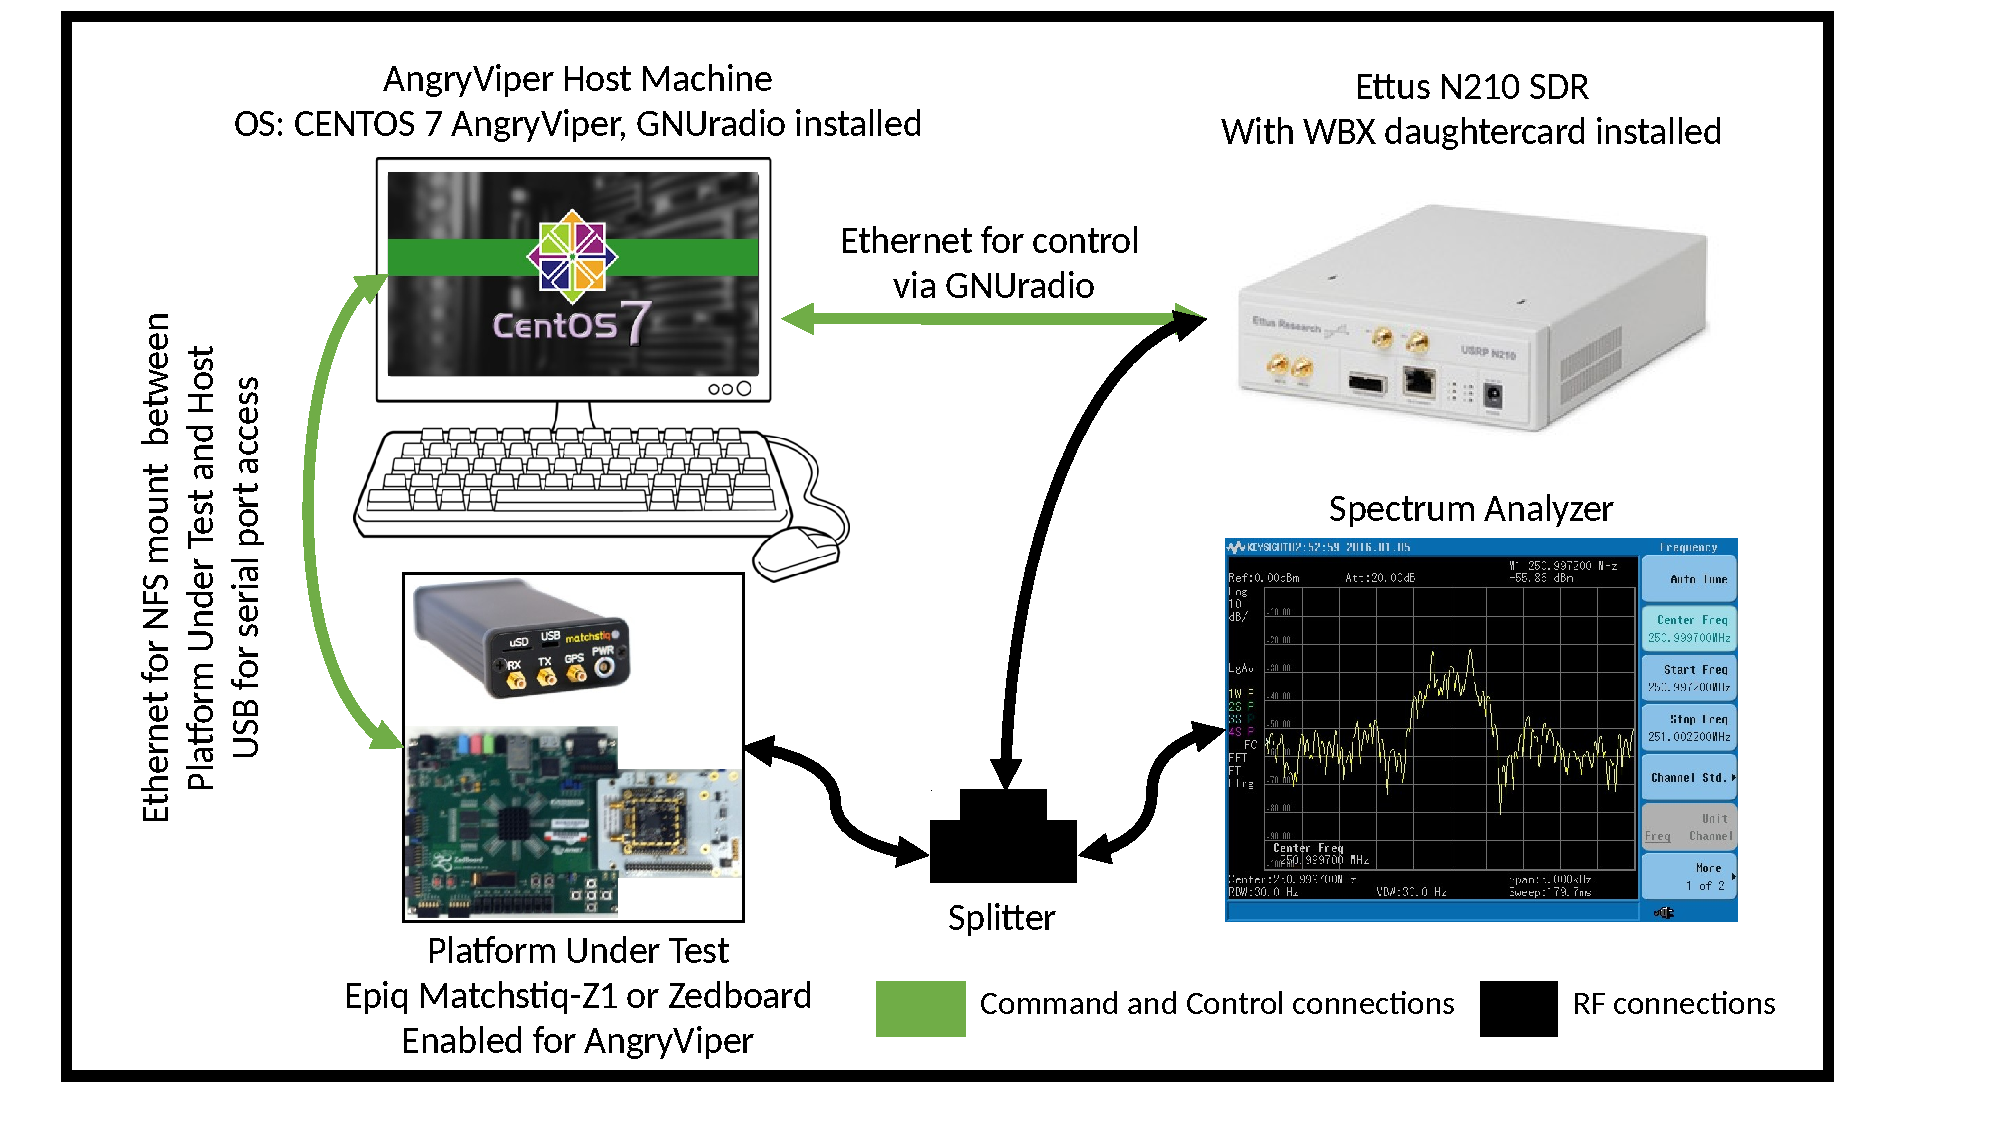
\includegraphics[scale=.55]{rx_app_test_setup}
		\caption{RX App Test Setup}
		\label{fig:rx_app_test_setup}
	\end{figure}
\subsection{make show}
\noindent In order to test the application, \texttt{make show} can be run from the \texttt{applications/rx\_app} directory. This provides instructions (for Zynq-Based Platforms) for setting \texttt{OCPI\_LIBRARY\_PATH} on the hardware platform and then running the application. Finally, it explains how to verify the output data on the development computer. The following sections provide further insight into these instructions.
\subsection{Artifacts}
\noindent Before running the application, the location of the required deployable artifacts must be specified in the OCPI\_LIBRARY\_PATH environment variable. Separate artifacts are needed for each RCC worker, and one artifact for the required FPGA image. Furthermore, artifacts differ depending on which mode the application is to be run in. Appendix B includes a list of the artifacts required for each platform and mode.
\subsection{Arguments to executable}
\noindent There are 9 arguments to the RX app executable. They primarily configure the RF front end of the Platform Unit Test using the matchstiq\_z1\_rx.rcc/zipper\_rx.rcc components. Additionally, the application can be configured by setting properties in the application XML file: rx\_app.xml. Descriptions of properties can be found in the individual component datasheets. Valid ranges for each argument can be printed out by running the executable with no arguments.\par\medskip
\noindent The arguments to the executable are summarized in the below table:
	\begin{center}
	\begin{tabularx}{\textwidth}{|c|C|}
	\hline
	\rowcolor{blue}
	Argument & Description\\
	\hline
	rf\_tune\_freq & RF (analog) tuning frequency in MHz\\
	\hline
	data\_bw & Effective sample rate of the frontend ADC (as well as the data being written to file) in MS/s\\
	\hline
	rf\_bw & Analog RF filter bandwidth in MHz\\
	\hline
	rf\_gain & RF (analog) gain in dB\\
	\hline
	bb\_bw & Analog filter bandwidth of the basebanded (downconverted) signal path in MHz\\
	\hline
	bb\_gain & Gain (analog) of basebanded (downconverted) signal path in dB\\
	\hline
	if\_tune\_freq & Tuning frequency in MHz of the HDL mixer which mixes (downconverts) the digitized data stream\\
	\hline
	runtime & Runtime of app in seconds\\
	\hline
	enable\_timestamps & Enable timestamp insertion in between messages\\
	\hline
	\end{tabularx}
	\end{center}
\subsection{Library Path Requirements}
\noindent Prior to running the application, the environment variable OCPI\_LIBRARY\_PATH must include the following directories:\par\medskip
\begin{minipage}[t]{.3\textwidth}
	\textbf{Matchstiq-Z1}
	\begin{itemize}
		\item ocpi library location
		\item ocpi.devices library location
		\item ocpi.assets.devices library location
		\item ocpi.assets.platforms.matchst-\\iq\_z1.devices library location
		\item ocpi.assets assemblies library location
	\end{itemize}
	\end{minipage}
\begin{minipage}[t]{.3\textwidth}
	\textbf{Zedboard with Zipper}
	\begin{itemize}
		\item ocpi library location
		\item ocpi.devices library location
		\item ocpi.assets.devices library location
		\item ocpi.assets assemblies library location
	\end{itemize}
	\end{minipage}
\begin{minipage}[t]{.3\textwidth}
	\textbf{Stratix IV GX230/ML605 with Zipper}
	\begin{itemize}
		\item ocpi.assets bitstream file location (first in path)
		\item ocpi library location
		\item ocpi.devices library location
		\item ocpi.assets.devices library location
	\end{itemize}
	\end{minipage}
	\par\bigskip\bigskip

\noindent Note that the Stratix IV GX230/Zipper/MyriadRF and ML605/Zipper/MyriadRF hardware setups require the intended slot-specific bitstream's file location to occur first in OCPI\_LIBRARY\_PATH. This is necessary because ocpirun's aritifact compatibility test can not currently differentiate between slot-connected device workers for multiple bitstreams that contain the same device worker, in the scenario where what differentiates the bitstreams is the device worker's slot connectivity. Examples of library paths that could be used can be seen below:\par\medskip
\noindent\textbf{Example Matchstiq-Z1 Library Path}\\
\verb|OCPI_LIBRARY_PATH=$PWD:$OCPI_CDK_DIR/../projects/core/lib/components:/mnt/ocpi_b| \\
\verb|aseproject/hdl/devices/lib/rcc/:/mnt/ocpi_assetshdl/devices/lib/rcc/:/mnt/ocpias| \\
\verb|sets/hdl/platforms/matchstiq z1/devices/lib/rcc/:../../hdl/assemblies/|
\par\medskip
\noindent\textbf{Example Zedboard/Zipper Library Path}\\
\verb|OCPI_LIBRARY_PATH=$PWD:$OCPI_CDK_DIR/../projects/core/lib/components:/mnt| \\
\verb|/ocpi_core/hdl/devices/lib/rcc/:/mnt/ocpi_assetshdl/devices/lib/rc| \\
\verb|c/:../../hdl/assemblies/|
\par\medskip
\noindent\textbf{Example Stratix IV GX230/Zipper in HSMC A Library Path}\\
\verb|OCPI_LIBRARY_PATH=../../hdl/assemblies/dc_offset_iq_imbalance_mixer_cic_dec_time| \\
\verb|stamper/container-dc_offset_iq_imbalance_mixer_cic_dec_timestamper_alst4_alst4_z| \\
\verb|ipper_hsmc_alst4_port_a_rx_rx_alst4_zipper_hsmc_a_thruassembly_container/target-| \\
\verb|stratix4/dc_offset_iq_imbalance_mixer_cic_dec_timestamper_alst4_alst4_zipper_hsm| \\
\verb|c_alst4_port_a_rx_rx_alst4_zipper_hsmc_a_thruassembly_container.bitz:$PWD:$OCPI_| \\
\verb|CDK_DIR/../projects/core/lib/components:/data/ocpi_core/hdl/devices/lib/r| \\
\verb|cc/:../../hdl/devices/lib/rcc/|
\par\medskip
\pagebreak
\noindent\textbf{Example Stratix IV GX230/Zipper in HSMC B Library Path}\\
\verb|OCPI_LIBRARY_PATH=../../hdl/assemblies/dc_offset_iq_imbalance_mixer_cic_dec_time| \\
\verb|stamper/container-dc_offset_iq_imbalance_mixer_cic_dec_timestamper_alst4_alst4_z| \\
\verb|ipper_hsmc_alst4_port_b_rx_rx_alst4_zipper_hsmc_b_thruassembly_container/target-| \\
\verb|stratix4/dc_offset_iq_imbalance_mixer_cic_dec_timestamper_alst4_alst4_zipper_hsm| \\
\verb|c_alst4_port_b_rx_rx_alst4_zipper_hsmc_b_thruassembly_container.bitz:$PWD:$OCPI_| \\
\verb|CDK_DIR/../projects/core/lib/components:/data/ocpi_core/hdl/devices/lib/r| \\
\verb|cc/:../../hdl/devices/lib/rcc/|
\par\medskip
\noindent\textbf{Example ML605/Zipper in FMC LPC Library Path}\\
\verb|OCPI_LIBRARY_PATH=../../hdl/assemblies/dc_offset_iq_imbalance_mixer_cic_dec_time| \\
\verb|stamper/container-dc_offset_iq_imbalance_mixer_cic_dec_timestamper_ml605_ml605_z| \\
\verb|ipper_fmc_lpc_rx_rx_ml605_zipper_fmc_lpc_thruassembly_container/target-virtex6/d| \\
\verb|c_offset_iq_imbalance_mixer_cic_dec_timestamper_ml605_ml605_zipper_fmc_lpc_rx_rx| \\
\verb|_ml605_zipper_fmc_lpc_thruassembly_container.bitz:$PWD:$OCPI_CDK_DIR/lib/compone| \\
\verb|nts:/data/ocpi_core/hdl/devices/lib/rcc/:../../hdl/devices/lib/rcc/|
\par\medskip
\noindent\textbf{Example ML605/Zipper in FMC HPC Library Path}\\
\verb|OCPI_LIBRARY_PATH=../../hdl/assemblies/dc_offset_iq_imbalance_mixer_cic_dec_time| \\
\verb|stamper/container-dc_offset_iq_imbalance_mixer_cic_dec_timestamper_ml605_ml605_z| \\
\verb|ipper_fmc_hpc_rx_rx_ml605_zipper_fmc_hpc_thruassembly_container/target-virtex6/d| \\
\verb|c_offset_iq_imbalance_mixer_cic_dec_timestamper_ml605_ml605_zipper_fmc_hpc_rx_rx| \\
\verb|_ml605_zipper_fmc_hpc_thruassembly_container.bitz:$PWD:$OCPI_CDK_DIR/lib/compone| \\
\verb|nts:/data/ocpi_core/hdl/devices/lib/rcc/:../../hdl/devices/lib/rcc/|
\pagebreak
\subsection{Expected results}
\noindent A python script is included with the application for plotting the received data in both the time and frequency domain. Using the test setup shown above and the default settings for the GNUradio FSK block diagram, run the application with the following arguments:\par\medskip
\noindent\textbf{Matchstiq-Z1}\\
\scriptsize
\begin{verbatim}
# Usage is:
# ./target-linux-x13_3-arm/rx_app rf_tune_freq data_bw rf_bw rf_gain bb_bw bb_gain if_tune_freq runtime enable_timestamps
  ./target-linux-x13_3-arm/rx_app 1000         0.256   400   10      0.75  51      0.256        1       1
\end{verbatim}
\par\medskip
\small

\noindent\textbf{Zedboard (with Zipper/Myriad RF card)}\\

\scriptsize
\begin{verbatim}
# Usage is:
# ./target-linux-x13_3-arm/rx_app rf_tune_freq data_bw rf_bw rf_gain bb_bw bb_gain if_tune_freq runtime enable_timestamps
  ./target-linux-x13_3-arm/rx_app 1000         0.256   -1    10      0.75  51      0.256        1       1
\end{verbatim}
\par\medskip
\small

\noindent\textbf{Stratix IV GX230 (with Zipper/Myriad RF card)}\\
\scriptsize
\noindent
\begin{verbatim}
# Usage is:
# ./target-linux-c6-x86_64/rx_app rf_tune_freq data_bw rf_bw rf_gain bb_bw bb_gain if_tune_freq runtime enable_timestamps
  ./target-linux-c6-x86_64/rx_app 1000         0.256   -1    6       0.75  51      0.256        1       1
\end{verbatim}
\small

\noindent\textbf{ML605 (with Zipper/Myriad RF card)}\\
\scriptsize
\noindent
\begin{verbatim}
# Usage is:
# ./target-linux-c6-x86_64/rx_app rf_tune_freq data_bw rf_bw rf_gain bb_bw bb_gain if_tune_freq runtime enable_timestamps
  ./target-linux-c6-x86_64/rx_app 1000         0.256   -1    6       0.75  51      0.256        1       1
\end{verbatim}
\small
\par\medskip
\noindent The output file can then be plotted with the python script with the following syntax and the output can be seen below:\par\medskip
\noindent\texttt{python ./scripts/plotAndFftAndTime.py odata/rx\_app\_raw.out complex 18000 256000 16352}\par
	\begin{figure}[h]
	 	\centering
		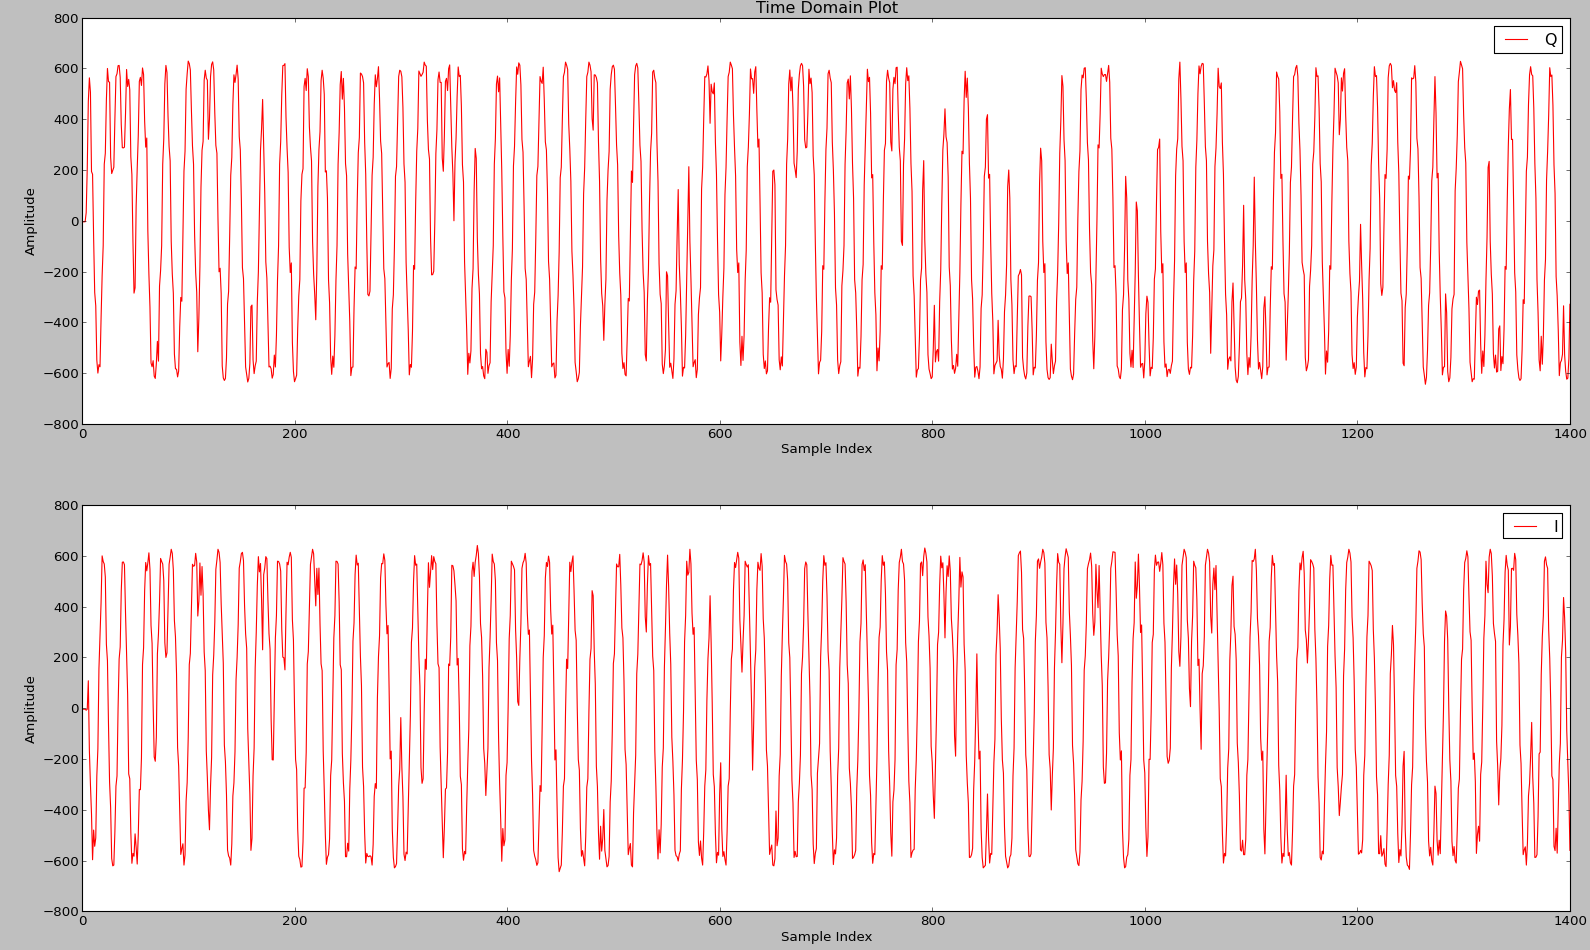
\includegraphics[scale=.2]{rx_app_iq_plot}
		\label{fig:rx_app_iq_plot}
	\end{figure}
	\begin{figure}[h]
	 	\centering
		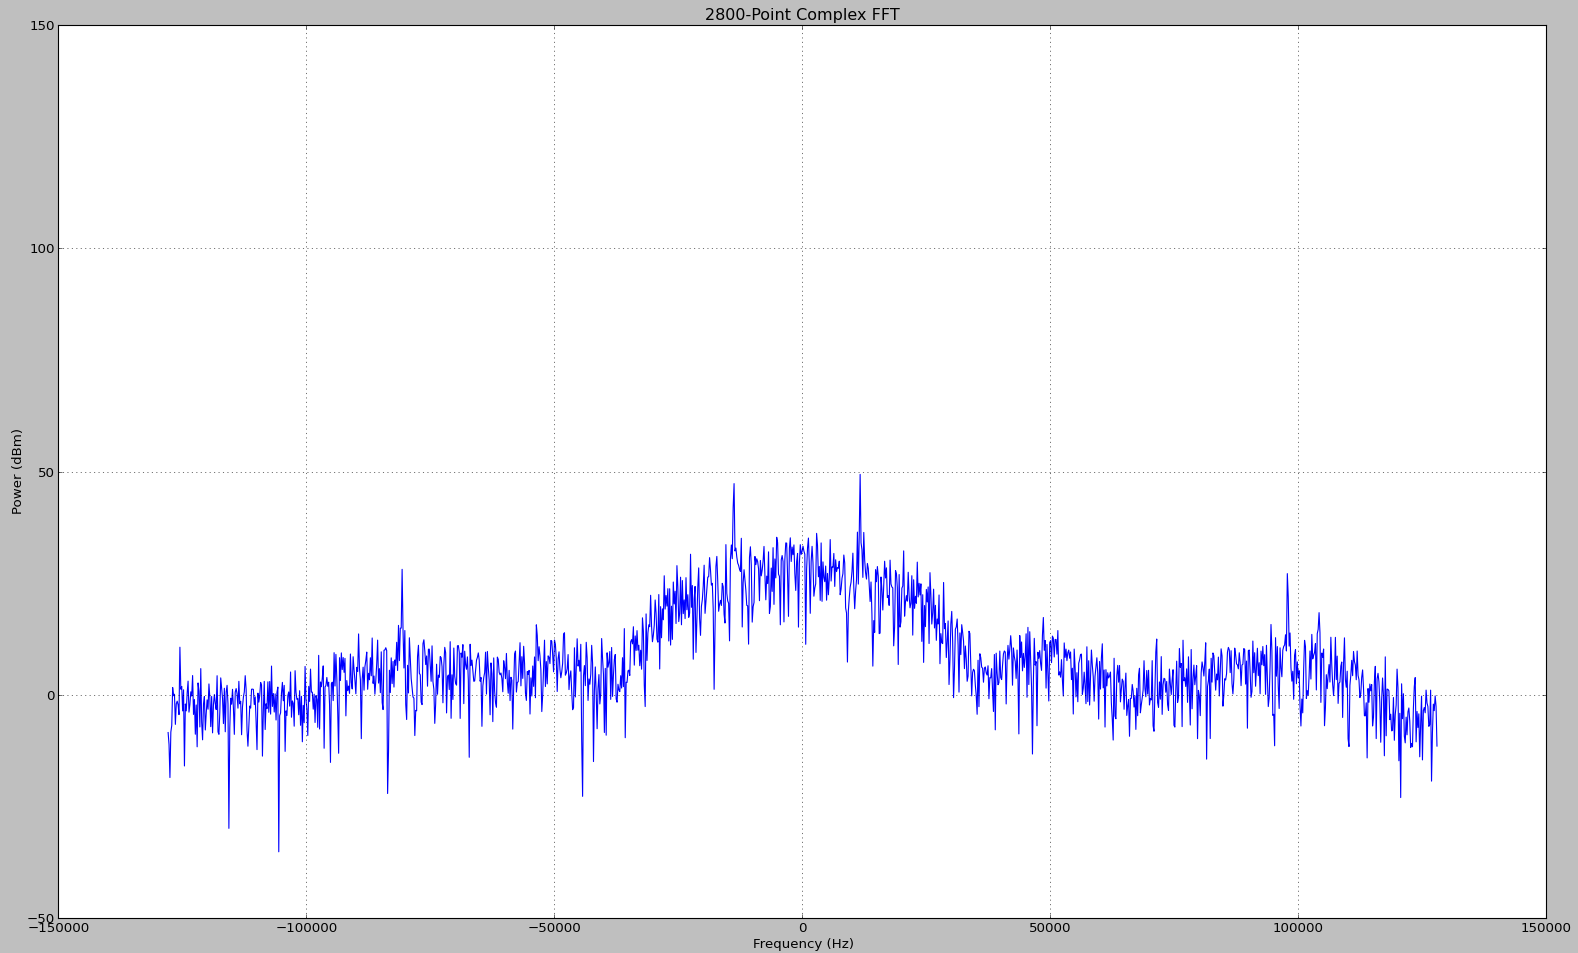
\includegraphics[scale=.2]{rx_app_fft_plot}
		\caption{Output of RX app}
		\label{fig:rx_app_fft_plot}
	\end{figure}
\noindent Alternatively, the shortened file can be plotted which will ignore potentially unwanted startup data:\par\medskip
\noindent\texttt{python ./scripts/plotAndFftAndTime.py odata/rx\_app\_shortened.out complex 18000 256000 16352}\par\medskip
\noindent The default sample rate for the GNUradio FSK block diagram is 512 kS/s. It is recommended that when using RX app with this input signal that a sample rate close to 512 kS/s be used. Higher sample rates are still valid, but may produce plots that look drastically different than those shown here.\par\medskip
\newpage
\noindent Timestamps are embedded, optionally, in the output file, and in addition to plotting, the script parses out and prints the timestamps. An example output gathered using the syntax above:\par\medskip
\scriptsize\noindent\texttt{Timestamp at index: 000000000 :  1.0728292 Seconds: 0x1 Fraction: 0x12a4eec4  \\
Timestamp at index: 000008180 :  1.0887978 Seconds: 0x1 Fraction: 0x16bb73ba ('Delta: 0.0159686', 'Expected:, 0.0159688')\\
Timestamp at index: 000016360 :  1.1047664 Seconds: 0x1 Fraction: 0x1ad1f906 ('Delta: 0.0159686', 'Expected:, 0.0159688')}\par\medskip
\noindent\small A small discrepancy (+/- 10) between Delta and Expected is typical. The difference is an artifact of the resolution of the fractional part of the timestamp applied in the timestamper HDL component. More information can be found in the timestamper component datasheet.\par\medskip
\par\medskip

\subsection{Using a RF Signal Generator}
\noindent As mentioned earlier, an arbitrary RF signal generator can be used with RX app instead of the Ettus N210. Below is an example using a signal generator and a Matchstiq-Z1 or Zed/Zipper.\par\medskip
\noindent In this example, the signal generator is set to 1.001250 GHz with an amplitude of -60 dBm (Matchstiq-Z1) or -40 dBm (Zed/Zipper). The following parameters can be passed to the executable:\par\medskip

\noindent\textbf{Matchstiq-Z1}\\
\scriptsize
\noindent
\begin{verbatim}
# Usage is:
# ./target-linux-x13_3-arm/rx_app rf_tune_freq data_bw rf_bw rf_gain bb_bw bb_gain if_tune_freq runtime enable_timestamps
  ./target-linux-x13_3-arm/rx_app 1000         2.5     400   10      1.25  51      1            1       1
\end{verbatim}
\par\medskip

\normalsize
\noindent\textbf{Zed/Zipper}\\
\scriptsize
\noindent
\begin{verbatim}
# Usage is:
# ./target-linux-x13_3-arm/rx_app rf_tune_freq data_bw rf_bw rf_gain bb_bw bb_gain if_tune_freq runtime enable_timestamps
  ./target-linux-x13_3-arm/rx_app 1000         2.5     -1   6      1.25  51      1            1       1
\end{verbatim}
\par\medskip
\small
\noindent Here we plot output data:\par\medskip
\noindent\texttt{python ./scripts/plotAndFftAndTime.py odata/rx\_app\_shortened.out complex 65536 2500000 16352}\par\medskip
\pagebreak
        \begin{figure}[h]
                \centering
                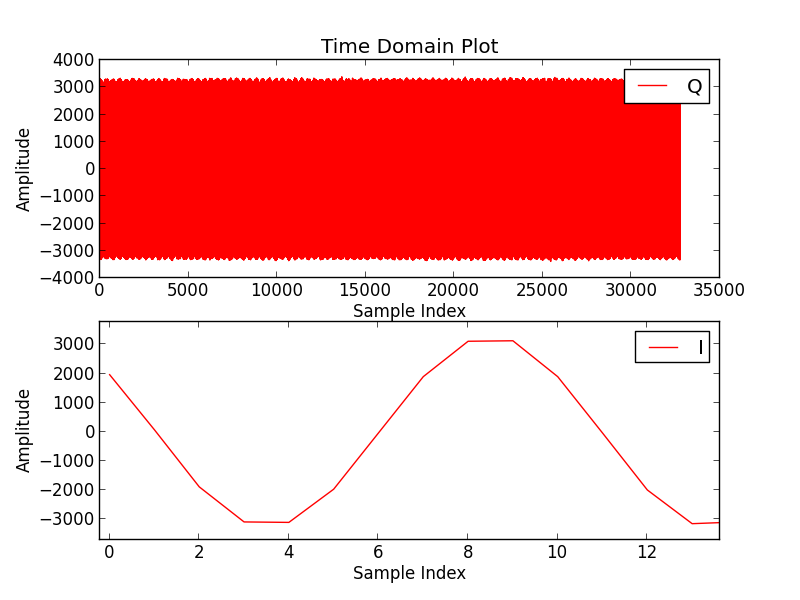
\includegraphics[scale=.5]{rx_app_sig_gen_time_domain}
                \label{fig:rx_app_sig_gen_time_domain}
        \end{figure}
        \begin{figure}[h]
                \centering
                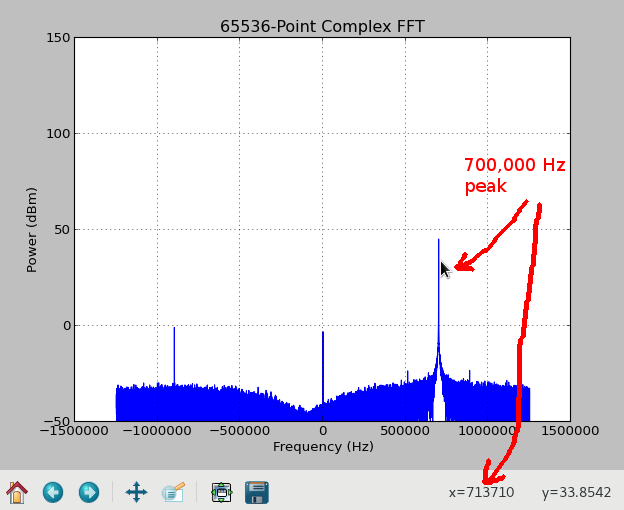
\includegraphics[scale=.5]{rx_app_sig_gen_fft}
                \caption{Output of RX app for Matchstiq-Z1}
                \label{fig:rx_app_sig_gen_fft}
        \end{figure}
\pagebreak
        \begin{figure}[h]
                \centering
                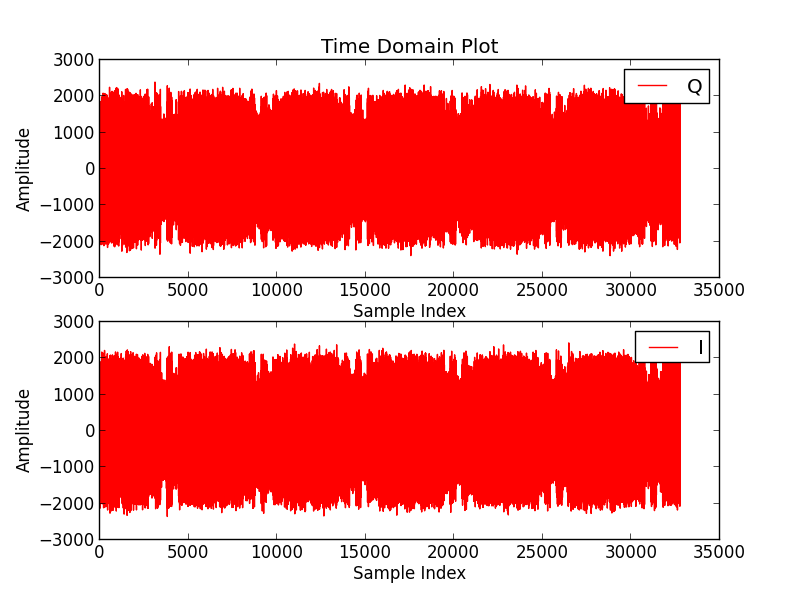
\includegraphics[scale=.5]{rx_app_sig_gen_time_domain_zed_zipper}
                \label{fig:rx_app_sig_gen_time_domain_zed_zipper}
        \end{figure}
        \begin{figure}[h]
                \centering
                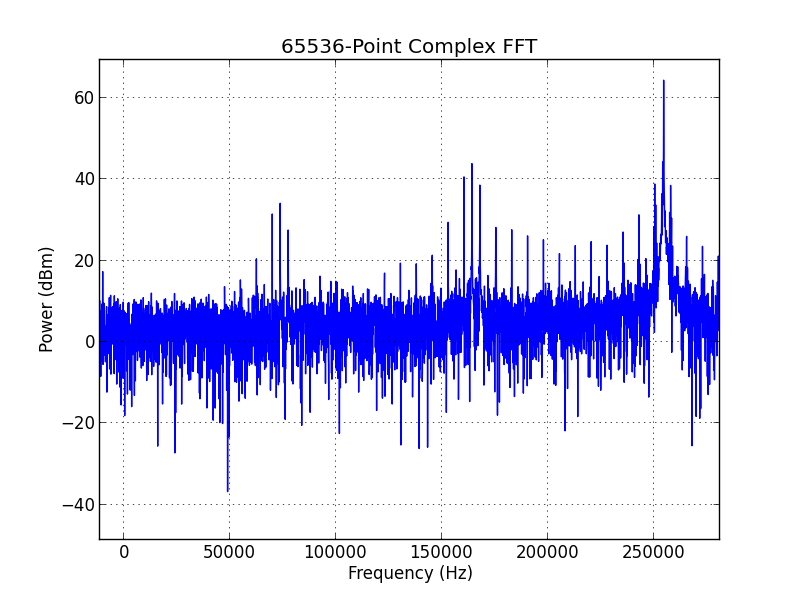
\includegraphics[scale=.5]{rx_app_sig_gen_fft_zed_zipper}
                \caption{Output of RX app for Zed/Zipper}
                \label{fig:rx_app_sig_gen_fft_zed_zipper}
        \end{figure}
\subsection{Known Limitations}
\noindent For more information on known limitations when using the Zipper-related platforms (Zedboard, Stratix IV, ML605), see the document Myriad-RF\_1\_Zipper\_Limitations included with this project.\pagebreak
\subsection{Known Issues}
If the path \path{/var/volatile} does not exist or requires root permission to write to, you will need to modify the ACI and the application XML to use a different directory for writing data. This involves simply finding and replacing \path{/var/volatile} with a different directory in the \path{.cxx} and \path{.xml} files. Failing to make this change when necessary may result in a segmentation fault error at application runtime.
% AV-3179
\section{Appendix A: Worker Parameters}
\begin{minipage}[t]{.5\textwidth}
	\textbf{Matchstiq-Z1}
	\begin{itemize}
		\item cic\_dec.hdl
			\subitem N = 3
			\subitem M = 1
			\subitem R = 8
			\subitem DIN\_WIDTH = 16
			\subitem ACC\_WIDTH = 25
			\subitem DOUT\_WIDTH = 16
		\item complex\_mixer.hdl
			\subitem NCO\_DATA\_WIDTH\_p = 12
			\subitem INPUT\_DATA\_WIDTH\_p = 12
			\subitem CORDIC\_STAGES\_p = 16
			\subitem PEAK\_MONITOR\_p = true
		\item iq\_imbalance\_fixer.hdl
			\subitem DATA\_WIDTH\_p = 16
			\subitem ACC\_PREC\_p = 34
			\subitem PEAK\_MONITOR\_p = true
		\item dc\_offset\_filter.hdl
			\subitem DATA\_WIDTH\_p = 16
			\subitem PEAK\_MONITOR\_p = true
		\item lime\_adc.hdl
			\subitem DRIVE\_CLK\_p = false
			\subitem USE\_CLK\_IN\_p = false
			\subitem USE\_CTL\_CLK\_p = false
			\subitem USE\_CLK\_OUT\_p = true
		\item si5338.hdl
			\subitem CLKIN\_PRESENT\_p = true
			\subitem CLKIN\_FREQ\_p = 3.072e7
			\subitem XTAL\_PRESENT\_p = false
			\subitem XTAL\_FREQ\_p = 0
			\subitem OUTPUTS\_PRESENT\_p = 1,0,0,0
			\subitem INTR\_CONNECTED\_p = false
		\item matchstiq\_z1\_i2c.hdl
			\subitem NUSERS\_p = 5
			\subitem SLAVE\_ADDRESS\_p = 0x45,0x71,0x48,0x21,0x20
			\subitem CLK\_CNT\_p = 199
	\end{itemize}
\end{minipage}
\begin{minipage}[t]{.5\textwidth}
	\textbf{Zedboard (with Zipper/Myriad-RF card)}
	\begin{itemize}
		\item cic\_dec.hdl
			\subitem N = 3
			\subitem M = 1
			\subitem R = 8
			\subitem DIN\_WIDTH = 16
			\subitem ACC\_WIDTH = 25
			\subitem DOUT\_WIDTH = 16
		\item complex\_mixer.hdl
			\subitem NCO\_DATA\_WIDTH\_p = 12
			\subitem INPUT\_DATA\_WIDTH\_p = 12
			\subitem CORDIC\_STAGES\_p = 16
			\subitem PEAK\_MONITOR\_p = true
		\item iq\_imbalance\_fixer.hdl
			\subitem DATA\_WIDTH\_p = 16
			\subitem ACC\_PREC\_p = 34
			\subitem PEAK\_MONITOR\_p = true
		\item dc\_offset\_filter.hdl
			\subitem DATA\_WIDTH\_p = 16
			\subitem PEAK\_MONITOR\_p = true
		\item lime\_adc.hdl
			\subitem DRIVE\_CLK\_p = false
			\subitem USE\_CLK\_IN\_p = true
			\subitem USE\_CTL\_CLK\_p = false
			\subitem USE\_CLK\_OUT\_p = false
		\item si5351.hdl
			\subitem CLKIN\_PRESENT = true
			\subitem CLKIN\_FREQ = 3.072e7
			\subitem XTAL\_PRESENT = false
			\subitem XTAL\_FREQ = 0
			\subitem VC\_PRESENT = false
			\subitem OUTPUTS\_PRESENT = 0,0,1,1,1,1,0,0
			\subitem OEB\_MODE = low
			\subitem INTR\_CONNECTED = false
		\item zipper\_i2c.hdl
			\subitem NUSERS\_p = 2
	\end{itemize}
\end{minipage}

\begin{minipage}[t]{.5\textwidth}
	\textbf{Stratix IV GX230 (with Zipper/Myriad-RF card)}
	\begin{itemize}
		\item cic\_dec.hdl
			\subitem N = 3
			\subitem M = 1
			\subitem R = 8
			\subitem DIN\_WIDTH = 16
			\subitem ACC\_WIDTH = 25
			\subitem DOUT\_WIDTH = 16
		\item complex\_mixer.hdl
			\subitem NCO\_DATA\_WIDTH\_p = 12
			\subitem INPUT\_DATA\_WIDTH\_p = 12
			\subitem CORDIC\_STAGES\_p = 16
			\subitem PEAK\_MONITOR\_p = true
		\item iq\_imbalance\_fixer.hdl
			\subitem DATA\_WIDTH\_p = 16
			\subitem ACC\_PREC\_p = 34
			\subitem PEAK\_MONITOR\_p = true
		\item dc\_offset\_filter.hdl
			\subitem DATA\_WIDTH\_p = 16
			\subitem PEAK\_MONITOR\_p = true
		\item lime\_adc.hdl
			\subitem DRIVE\_CLK\_p = false
			\subitem USE\_CLK\_IN\_p = true
			\subitem USE\_CTL\_CLK\_p = false
			\subitem USE\_CLK\_OUT\_p = false
		\item si5351.hdl
			\subitem CLKIN\_PRESENT = true
			\subitem CLKIN\_FREQ = 3.072e7
			\subitem XTAL\_PRESENT = false
			\subitem XTAL\_FREQ = 0
			\subitem VC\_PRESENT = false
			\subitem OUTPUTS\_PRESENT = 0,0,1,1,1,1,0,0
			\subitem OEB\_MODE = low
			\subitem INTR\_CONNECTED = false
		\item zipper\_i2c.hdl
			\subitem NUSERS\_p = 2
	\end{itemize}
\end{minipage}
\begin{minipage}[t]{.5\textwidth}
	\textbf{ML605 (with Zipper/Myriad-RF card)}
	\begin{itemize}
		\item cic\_dec.hdl
			\subitem N = 3
			\subitem M = 1
			\subitem R = 8
			\subitem DIN\_WIDTH = 16
			\subitem ACC\_WIDTH = 25
			\subitem DOUT\_WIDTH = 16
		\item complex\_mixer.hdl
			\subitem NCO\_DATA\_WIDTH\_p = 12
			\subitem INPUT\_DATA\_WIDTH\_p = 12
			\subitem CORDIC\_STAGES\_p = 16
			\subitem PEAK\_MONITOR\_p = true
		\item iq\_imbalance\_fixer.hdl
			\subitem DATA\_WIDTH\_p = 16
			\subitem ACC\_PREC\_p = 34
			\subitem PEAK\_MONITOR\_p = true
		\item dc\_offset\_filter.hdl
			\subitem DATA\_WIDTH\_p = 16
			\subitem PEAK\_MONITOR\_p = true
		\item lime\_adc.hdl
			\subitem DRIVE\_CLK\_p = false
			\subitem USE\_CLK\_IN\_p = true
			\subitem USE\_CTL\_CLK\_p = false
			\subitem USE\_CLK\_OUT\_p = false
		\item si5351.hdl
			\subitem CLKIN\_PRESENT = true
			\subitem CLKIN\_FREQ = 3.072e7
			\subitem XTAL\_PRESENT = false
			\subitem XTAL\_FREQ = 0
			\subitem VC\_PRESENT = false
			\subitem OUTPUTS\_PRESENT = 0,0,1,1,1,1,0,0
			\subitem OEB\_MODE = low
			\subitem INTR\_CONNECTED = false
		\item zipper\_i2c.hdl
			\subitem NUSERS\_p = 2
	\end{itemize}
\end{minipage}\newpage

\section{Appendix B: Artifacts}
\subsection{Matchstiq-Z1}
	\begin{itemize}
	\item dc\_offset\_iq\_imbalance\_mixer\_cic\_dec\_timestamper\_matchstiq\_z1\_matchstiq\_z1\_rx\_rx\_matchstiq\_z1\_container.bitz
	\end{itemize}
	\begin{itemize}
	\begin{minipage}[t]{.5\textwidth}
	\item target-linux-x13\_3-arm/file\_write\_s.so
	\item target-linux-x13\_3-arm/matchstiq\_z1\_rx\_s.so
	\item target-linux-x13\_3-arm/matchstiq\_z1\_tx\_s.so
	\item target-linux-x13\_3-arm/lime\_rx\_proxy\_s.so
	\item target-linux-x13\_3-arm/lime\_tx\_proxy\_s.so
	\end{minipage}
	\begin{minipage}[t]{.5\textwidth}
	\item target-linux-x13\_3-arm/si5338\_proxy\_s.so
	\item target-linux-x13\_3-arm/matchstiq\_z1\_avr\_proxy\_s.so
	\item target-linux-x13\_3-arm/tmp100\_proxy\_s.so
	\item target-linux-x13\_3-arm/matchstiq\_z1\_pca9535\_proxy\_s.so
	\end{minipage}
	\end{itemize}
\subsection{Zedboard}
	\begin{itemize}
	\item dc\_offset\_iq\_imbalance\_mixer\_cic\_dec\_timestamper\_zed\_base\_rx\_zed\_zipper\_container.bitz
	\end{itemize}
	\begin{itemize}
	\begin{minipage}[t]{.5\textwidth}
	\item target-linux-x13\_3-arm/file\_write\_s.so
	\item target-linux-x13\_3-arm/zipper\_rx\_s.so
	\item target-linux-x13\_3-arm/zipper\_tx\_s.so
	\end{minipage}
	\begin{minipage}[t]{.5\textwidth}
	\item target-linux-x13\_3-arm/lime\_rx\_proxy\_s.so
	\item target-linux-x13\_3-arm/lime\_tx\_proxy\_s.so
	\item target-linux-x13\_3-arm/si5351\_proxy\_s.so
	\end{minipage}
	\end{itemize}
\subsection{Stratix IV}
	\begin{itemize}
	\begin{minipage}[t]{.5\textwidth}
	\item target-linux-c7-x86\_64/file\_read\_s.so
	\item target-linux-c7-x86\_64/zipper\_rx\_s.so
	\item target-linux-c7-x86\_64/zipper\_tx\_s.so
	\end{minipage}
	\begin{minipage}[t]{.5\textwidth}
	\item target-linux-c7-x86\_64/lime\_rx\_proxy\_s.so
	\item target-linux-c7-x86\_64/lime\_tx\_proxy\_s.so
	\item target-linux-c7-x86\_64/si5351\_proxy\_s.so
	\end{minipage}
	\end{itemize}
	For Zipper plugged into HSMC Port A:
	\begin{itemize}
		\item dc\_offset\_iq\_imbalance\_mixer\_cic\_dec\_timestamper\_alst4\_alst4\_zipper\_hsmc\_alst4\_port\_a\_rx\_rx\_alst4\_zipper\_hsmc\_a\\ \_thruassembly\_container.bitz
	\end{itemize}
	\noindent For Zipper plugged into HSMC Port B:
	\begin{itemize}
		\item dc\_offset\_iq\_imbalance\_mixer\_cic\_dec\_timestamper\_alst4\_alst4\_zipper\_hsmc\_alst4\_port\_b\_rx\_rx\_alst4\_zipper\_hsmc\_b\\ \_thruassembly\_container.bitz
	\end{itemize}
\subsection{ML605}
	\begin{itemize}
	\begin{minipage}[t]{.5\textwidth}
	\item target-linux-c7-x86\_64/file\_read\_s.so
	\item target-linux-c7-x86\_64/zipper\_rx\_s.so
	\item target-linux-c7-x86\_64/zipper\_tx\_s.so
	\end{minipage}
	\begin{minipage}[t]{.5\textwidth}
	\item target-linux-c7-x86\_64/lime\_rx\_proxy\_s.so
	\item target-linux-c7-x86\_64/lime\_tx\_proxy\_s.so
	\item target-linux-c7-x86\_64/si5351\_proxy\_s.so
	\end{minipage}
	\end{itemize}
	For Zipper plugged into FMC HPC:
	\begin{itemize}
		\item dc\_offset\_iq\_imbalance\_mixer\_cic\_dec\_timestamper\_ml605\_ml605\_zipper\_fmc\_hpc\_rx\_rx\_ml605\_zipper\_fmc\_hpc\\ \_thruassembly\_container.bitz
	\end{itemize}
	\noindent For Zipper plugged into FMC LPC:
	\begin{itemize}
		\item dc\_offset\_iq\_imbalance\_mixer\_cic\_dec\_timestamper\_ml605\_ml605\_zipper\_fmc\_lpc\_rx\_rx\_ml605\_zipper\_fmc\_lpc\\ \_thruassembly\_container.bitz
	\end{itemize}
\end{document}
